\title{Computer Architecture - CS 301} % You may change the title if you want.

\author{Rishit Saiya - 180010027, Assignment - 1 }

\date{\today}

\documentclass[12pt]{article}
\usepackage{fullpage}
\usepackage{enumitem}
\usepackage{amsmath,mathtools}
\usepackage{amssymb}
\usepackage[super]{nth}
\usepackage{textcomp}
\usepackage{hyperref}
\begin{document}
\maketitle

\section{}

\begin{enumerate}[label=(\alph*)]
    \item \textbf{2’s complementary method for signed integers} \\
    The general representation of a binary number with n bit is $n_1n_2n_3..n_n$ where $n_i$ where i $\in$ \{0,1\}. \\
    \textbf{For example:} $5$ in Binary Representation is denoted as $101$.
    
\textbf{Method-1 : Using 2's Complement} \\
    Now when we talk about Signed Integers, its different. If we are converting a positive number, the binary representation remains same. If its negative, then we calculate the binary of $2^{n} - |u|$, where we want to find binary representation of $-u$. \\
    \textbf{For example:} $-5$ in Binary Representation is denoted as $1011$ in a 4-bit Binary system because $2^{4} - |5|$ = 11 and its binary is 1011. 
    
\textbf{Method-2 : Using 1's Complement} \\    
    A 2's Complement for such can be calculated by many ways among which the most easy one is by 1's complement. In such methods we just invert the bits of signed binary representation and add 1, the resulting binary representation is called the 2's Complement for Signed Integers.
    
    \textbf{For example:}\\
            2's Complement of 5: \\
            Binary is 101 -$>$ Inverting the bits: 010 -$>$ 2's complement: 011 (Adding 1 to 010). \\
            2's Complement of -5:  \\
            Binary is 1011 -$>$ Inverting the bits: 0100 -$>$ 2's complement: 0101 (Adding 1 to 0100).
    
    \item \textbf{Cons of usage of solely signed bit for representation}\\
    The notion where one bit is the sign bit and the rest of the bits represent the magnitude of the integer isn't very feasible because of following reasons:
    \begin{itemize}
        \item The representation at zero isn't continuous and we would have 2 representations of $0$ (zero) always. \\
    \textbf{For example:} For a 4 bit representation, $0$ can be represented as $0000$ or $1000$. So ambiguity exists.
    \item The arithmetic operations like Addition and Subtraction become inaccurate in such cases. \\
    \textbf{For example:} Let's consider the operation: 5 + (-2) \\
    Signed Binary Representation of 5 $\rightarrow$ 0101 \\
    Signed Binary Representation of 2 $\rightarrow$ 1010 \\
    Operation: \\
    \begin{equation*}
        0101 + 1010 = 1111
    \end{equation*}
    Actually the operation should result 0011, but we got 1111 (15) instead, which is false.
    \end{itemize}
\end{enumerate}

\section{}
As given the in the Figure 1, we have to convert $X$ = -2.25 into IEEE 754 format.
    \begin{figure}
    \centering
    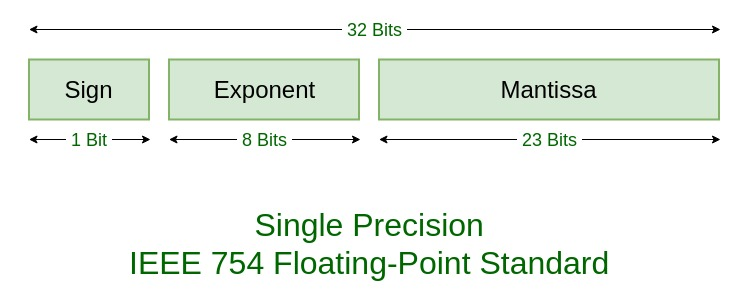
\includegraphics[width=15cm, height=5cm]{Single-Precision-IEEE-754-Floating-Point-Standard.png}
    \caption{IEEE 754 Floating Point Representation 32 bit}
\end{figure}
    The above figure gives us breakage of bits required in each slot.\\
    Since, X is negative, the sign bit is \textbf{1}.\\
    % The expansion of -2.25 is $2^1$ + $2^{-2}$. So the corresponding binary of -2.25 becomes 10.01.
    We need to find the E \& M for IEEE 754 notation. Hence, we convert it according to given exponential format as follows:\\
    
    \begin{equation*}
        X = (-1)^S \times P \times 2^{E-Bias}
    \end{equation*}
    where, Bias = 127 \& P = 1 + M.\\
    So, now for X = -2.25, the representation becomes: \\
    \begin{equation*}
        X = (-1)^1 \times 1.125 \times 2^{1}
    \end{equation*}
    Clearly \textbf{E = 127+1 = 128}. In binary representation, E becomes 10000000 (8-bits). \\
    Here P = 1.125 \& P = 1 + M, hence \textbf{M = 0.125}. In binary representation M becomes 001 because 0.125 = $2^{-3}$.
    
    So, IEEE 754 Format Representation (32-bit) becomes:
    \begin{center}
        \textbf{1 10000000 00100000000000000000000}    
    \end{center}
    
For the Hex Representation, we just group them into four bits and find the Hex equivalent of it and we get \textbf{C0100000}.

\section{}
    
     To reduce the loss of precision when an underflow occurs, IEEE 754 includes the ability to represent fractions smaller than are possible in the normalized representation, by making the implicit leading digit as 0. Hence the number before the decimal point becomes 0 instead of 1. Such numbers are called Denormal Numbers.\\
    
    The standard representation is:
    \begin{equation*}
        A = (-1)^S \times P \times 2^{-126}
    \end{equation*}
    where P = (0 + M), 0 $\leq$ M $<$ 1 \\

    The significand of this above form is : 0.XXXX. Also E = 0, X = -126.
    
    Largest Positive Denormal(LPD) number is as follows: 
    \begin{equation*}
        X_{LPD} = 0.11...11 (23 \, bits) \times 2^{-126}
    \end{equation*}
    \begin{equation*}
        X_{LPD} = (1-2^{-23}) \times 2^{-126}
    \end{equation*}
    \begin{equation*}
        X_{LPD} = 2^{-126} - 2^{-149}
    \end{equation*}
    
    Smallest Positive Denormal(SPD) number is as follows: 
    \begin{equation*}
        X_{SPD} = 0.00...01 (23 \, bits) \times 2^{-126}
    \end{equation*}
    \begin{equation*}
        X_{SPD} = (2^{-23}) \times 2^{-126}
    \end{equation*}
    \begin{equation*}
        X_{SPD} = (2^{-149})
    \end{equation*}
    
    Denormal numbers provide the guarantee that addition and subtraction of floating-point numbers never underflows: two nearby floating-point numbers always have a representable non-zero difference. Without gradual underflow, the subtraction (a - b) can underflow and produce zero even though the values are not equal.

\end{document}